% This file was created by matlab2tikz.
%
%The latest updates can be retrieved from
%  http://www.mathworks.com/matlabcentral/fileexchange/22022-matlab2tikz-matlab2tikz
%where you can also make suggestions and rate matlab2tikz.
%
\documentclass[tikz]{standalone}
\usepackage[T1]{fontenc}
\usepackage[utf8]{inputenc}
\usepackage{pgfplots}
\usepackage{grffile}
\pgfplotsset{compat=newest}
\usetikzlibrary{plotmarks}
\usetikzlibrary{arrows.meta}
\usetikzlibrary{spy}
\usepgfplotslibrary{patchplots}
\usepackage{amsmath}

\begin{document}
\definecolor{mycolor1}{rgb}{0.00000,0.44700,0.74100}%
%
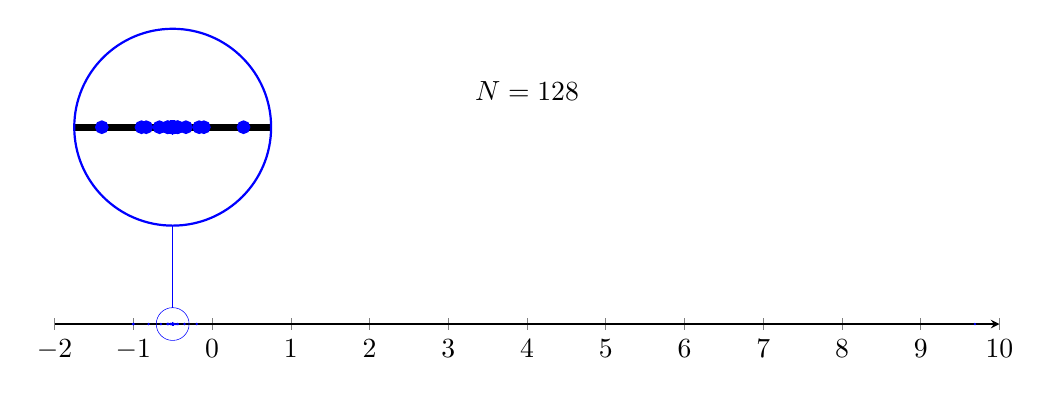
\begin{tikzpicture}[spy using outlines=
	{circle, magnification=6, connect spies}]

\begin{axis}[%
width=12cm,
height=3cm,
at={(0cm,0cm)},
scale only axis,
xmin=-2.000,
xmax=10.000,
ymin=-0.01,
ymax=0.05,
axis y line=none,
axis x line=middle,
axis background/.style={fill=white},
title={$N=128$}
]
\addplot [color=blue, draw=none, mark=*,mark options={scale=0.1}]
  table[row sep=crcr]{%
9.688	0\\
-1.000	0\\
-0.806	0\\
-0.194	0\\
-0.350	0\\
-1.000	0\\
-1.000	0\\
-0.650	0\\
-0.566	0\\
-0.556	0\\
-0.434	0\\
-0.444	0\\
-0.472	0\\
-0.528	0\\
-0.511	0\\
-0.490	0\\
-0.489	0\\
-0.510	0\\
-0.496	0\\
-0.504	0\\
-0.502	0\\
-0.502	0\\
-0.498	0\\
-0.498	0\\
-0.499	0\\
-0.499	0\\
-0.501	0\\
-0.501	0\\
-0.500	0\\
-0.500	0\\
-0.500	0\\
-0.500	0\\
-0.500	0\\
-0.500	0\\
-0.500	0\\
-0.500	0\\
-0.500	0\\
-0.500	0\\
-0.500	0\\
-0.500	0\\
-0.500	0\\
-0.500	0\\
-0.500	0\\
-0.500	0\\
-0.500	0\\
-0.500	0\\
-0.500	0\\
-0.500	0\\
-0.500	0\\
-0.500	0\\
-0.500	0\\
-0.500	0\\
-0.500	0\\
-0.500	0\\
-0.500	0\\
-0.500	0\\
-0.500	0\\
-0.500	0\\
-0.500	0\\
-0.500	0\\
-0.500	0\\
-0.500	0\\
-0.500	0\\
-0.500	0\\
-0.500	0\\
-0.500	0\\
-0.500	0\\
-0.500	0\\
-0.500	0\\
-0.500	0\\
-0.500	0\\
-0.500	0\\
-0.500	0\\
-0.500	0\\
-0.500	0\\
-0.500	0\\
-0.500	0\\
-0.500	0\\
-0.500	0\\
-0.500	0\\
-0.500	0\\
-0.500	0\\
-0.500	0\\
-0.500	0\\
-0.500	0\\
-0.500	0\\
-0.500	0\\
-0.500	0\\
-0.500	0\\
-0.500	0\\
-0.500	0\\
-0.500	0\\
-0.500	0\\
-0.500	0\\
-0.500	0\\
-0.500	0\\
-0.500	0\\
-0.500	0\\
-0.500	0\\
-0.500	0\\
-0.500	0\\
-0.500	0\\
-0.500	0\\
-0.500	0\\
-0.500	0\\
-0.500	0\\
-0.500	0\\
-0.500	0\\
-0.500	0\\
-0.500	0\\
-0.500	0\\
-0.500	0\\
-0.500	0\\
-0.500	0\\
-0.500	0\\
-0.500	0\\
-0.500	0\\
-0.500	0\\
-0.500	0\\
-0.500	0\\
-0.500	0\\
-0.500	0\\
-0.500	0\\
-0.500	0\\
-0.500	0\\
-0.500	0\\
-0.500	0\\
-0.500	0\\
-0.500	0\\
-0.500	0\\
-0.500	0\\
-0.500	0\\
-0.500	0\\
-0.500	0\\
-0.500	0\\
-0.500	0\\
-0.500	0\\
-0.500	0\\
-0.500	0\\
-0.500	0\\
-0.500	0\\
-0.500	0\\
-0.500	0\\
-0.500	0\\
-0.500	0\\
-0.500	0\\
-0.500	0\\
-0.500	0\\
-0.500	0\\
-0.500	0\\
-0.500	0\\
-0.500	0\\
-0.500	0\\
-0.500	0\\
-0.500	0\\
-0.500	0\\
-0.500	0\\
-0.500	0\\
-0.500	0\\
-0.500	0\\
-0.500	0\\
-0.500	0\\
-0.500	0\\
-0.500	0\\
-0.500	0\\
-0.500	0\\
-0.500	0\\
-0.500	0\\
-0.500	0\\
-0.500	0\\
-0.500	0\\
-0.500	0\\
-0.500	0\\
-0.500	0\\
-0.500	0\\
-0.500	0\\
-0.500	0\\
-0.500	0\\
-0.500	0\\
-0.500	0\\
-0.500	0\\
-0.500	0\\
-0.500	0\\
-0.500	0\\
-0.500	0\\
-0.500	0\\
-0.500	0\\
-0.500	0\\
-0.500	0\\
-0.500	0\\
-0.500	0\\
-0.500	0\\
-0.500	0\\
-0.500	0\\
-0.500	0\\
-0.500	0\\
-0.500	0\\
-0.500	0\\
-0.500	0\\
-0.500	0\\
-0.500	0\\
-0.500	0\\
-0.500	0\\
-0.500	0\\
-0.500	0\\
-0.500	0\\
-0.500	0\\
-0.500	0\\
-0.500	0\\
-0.500	0\\
-0.500	0\\
-0.500	0\\
-0.500	0\\
-0.500	0\\
-0.500	0\\
-0.500	0\\
-0.500	0\\
-0.500	0\\
-0.500	0\\
-0.500	0\\
-0.500	0\\
-0.500	0\\
-0.500	0\\
-0.500	0\\
-0.500	0\\
-0.500	0\\
-0.500	0\\
-0.500	0\\
-0.500	0\\
-0.500	0\\
-0.500	0\\
-0.500	0\\
-0.500	0\\
-0.500	0\\
-0.500	0\\
-0.500	0\\
-0.500	0\\
-0.500	0\\
-0.500	0\\
-0.500	0\\
-0.500	0\\
-0.500	0\\
-0.500	0\\
-0.500	0\\
-0.500	0\\
-0.500	0\\
-0.500	0\\
-0.500	0\\
-0.500	0\\
-0.500	0\\
-0.500	0\\
-0.500	0\\
-0.500	0\\
-0.500	0\\
-0.500	0\\
-0.500	0\\
};
  \coordinate (spypoint1) at (axis cs:-0.5,0);
  \coordinate (magnifyglass1) at (axis cs:-0.5,0.05);

\end{axis}

\spy [blue, size=2.5cm] on (spypoint1)  in node[fill=white] at (magnifyglass1);

\end{tikzpicture}%
\end{document}
\end{axis}
\end{tikzpicture}%
\end{document}